\documentclass[10pt]{beamer}

\usetheme[progressbar=frametitle]{metropolis}
\usepackage{appendixnumberbeamer}

\usepackage{booktabs}
\usepackage[scale=2]{ccicons}

\usepackage{pgfplots}
\usepgfplotslibrary{dateplot}

\usepackage{xspace}
\newcommand{\themename}{\textbf{\textsc{metropolis}}\xspace}


\title{A Survey of Multi-hop Reading Comprehension approaches using Graph Neural Networks}
\subtitle{Seminar Presentation}
% \date{\today}
\date{}

\author{Ajay Narayanan, Constantin Weberpals, Tim Bruckdorfer}

\institute{Technical University of Munich}
% \titlegraphic{\hfill\includegraphics[height=1.5cm]{logo.pdf}}

\begin{document}

\maketitle

\begin{frame}{Table of contents}
  \setbeamertemplate{section in toc}[sections numbered]
  \tableofcontents[hideallsubsections]
\end{frame}

\section[Intro]{Introduction}

\begin{frame}[fragile]{What is Multi-hop Reading Comprehension?}

  % The \themename theme is a Beamer theme with minimal visual noise
  % inspired by the \href{https://github.com/hsrmbeamertheme/hsrmbeamertheme}{\textsc{hsrm} Beamer
  % Theme} by Benjamin Weiss.

  % Enable the theme by loading

  % \begin{verbatim}    \documentclass{beamer}
  %   \usetheme{metropolis}\end{verbatim}

  % Note, that you have to have Mozilla's \emph{Fira Sans} font and XeTeX
  % installed to enjoy this wonderful typography.
  \begin{itemize}
    \item Machine reading comprehension is a task in NLP where a machine is given a question and a passage of text and is expected to answer the question using the passage.
    \item For Multi-hop RC, There are multiple passages, and the questions are usually complex and require the machine to perform multiple steps of reasoning to arrive at the answer.
    
  \end{itemize}
\end{frame}

\begin{frame}
  \begin{figure}[t] % 'h' for "here", can be replaced with other placement specifiers
    \centering
    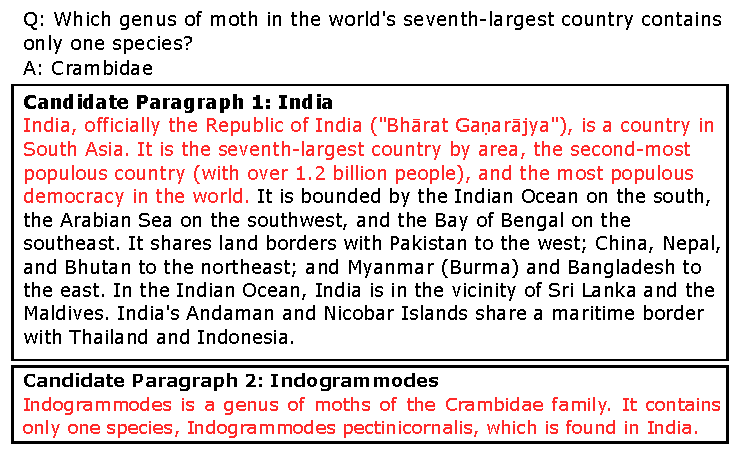
\includegraphics[width=\linewidth]{fig/fig_1_hotpot_example.pdf} % Adjust 'width' as needed
    \caption{A Sample question from the HotpotQA dataset}
    \label{fig:sample_hotpotqa} % For referencing the figure in the text
  \end{figure}
\end{frame}

\begin{frame}[fragile]{What is Multi-hop Reading Comprehension?}

  \begin{itemize}
    \item The task is usually split into two parts: finding the relevant parts of the passage and then using those parts to answer the question.
    \item The task is usually evaluated using the F1 score, which is the harmonic mean of precision and recall.
    \item Applications: Document summarization, complex query answering
    
  \end{itemize}
\end{frame}


% \begin{frame}[fragile]{Sections}
%   Sections group slides of the same topic

%   \begin{verbatim}    \section{Elements}\end{verbatim}

%   for which \themename provides a nice progress indicator \ldots
  
% \end{frame}

\section{Theoretical Background}

\subsection{Graph Neural Networks in MHRC}

\begin{frame}{Introduction to Graph Neural Networks in MHRC}
  \begin{itemize}
    \item GNNs adapt traditional neural network models to handle graph-structured data. [Scarselli et al., 2008] \cite{RN203}
    \item They capture complex relationships and interdependencies within data, making them ideal for MHRC tasks.
    \item Key features include node representation, where each node corresponds to an entity or a concept in the text.
    \item Neighborhood aggregation allows GNNs to gather and process information from connected nodes, essential for understanding context in MHRC.
    \item Iterative learning through these features enables GNNs to effectively model and reason over complex information networks. [Zhou et al., 2020] \cite{RN1}
  \end{itemize}
\end{frame}


\begin{frame}{GNN Variants and Their Application in MHRC}
  \begin{itemize}
    \item Graph Convolutional Networks (GCNs): Introduced by Kipf and Welling (2016), they generalize convolutional neural networks to graph data, making them adept at feature extraction for MHRC \cite{RN209}
    \item Graph Attention Networks (GATs): Proposed by Veličković et al. (2018), these networks use attention mechanisms to focus on important nodes, enhancing reasoning over graphs \cite{RN7}
    \item Application in MHRC: 
      \begin{itemize}
        \item GNNs, particularly GCNs and GATs, are effective in multi-hop reasoning tasks where information is scattered across different documents [De Cao et al., 2019] \cite{RN117}
        \item They excel at aggregating information from various sources, providing a structured way to approach complex questions in MHRC datasets [Yao et al., 2019]
      \end{itemize}
  \end{itemize}
\end{frame}


\subsection{Importance of Datasets}

\begin{frame}{Datasets in MHRC}
  \begin{itemize}
    \item Critical role in benchmarking performance and challenging reasoning capabilities.
    \item Example Datasets:
  \end{itemize}

  \begin{figure}[t] % 'h' for "here", can be replaced with other placement specifiers
    \centering
    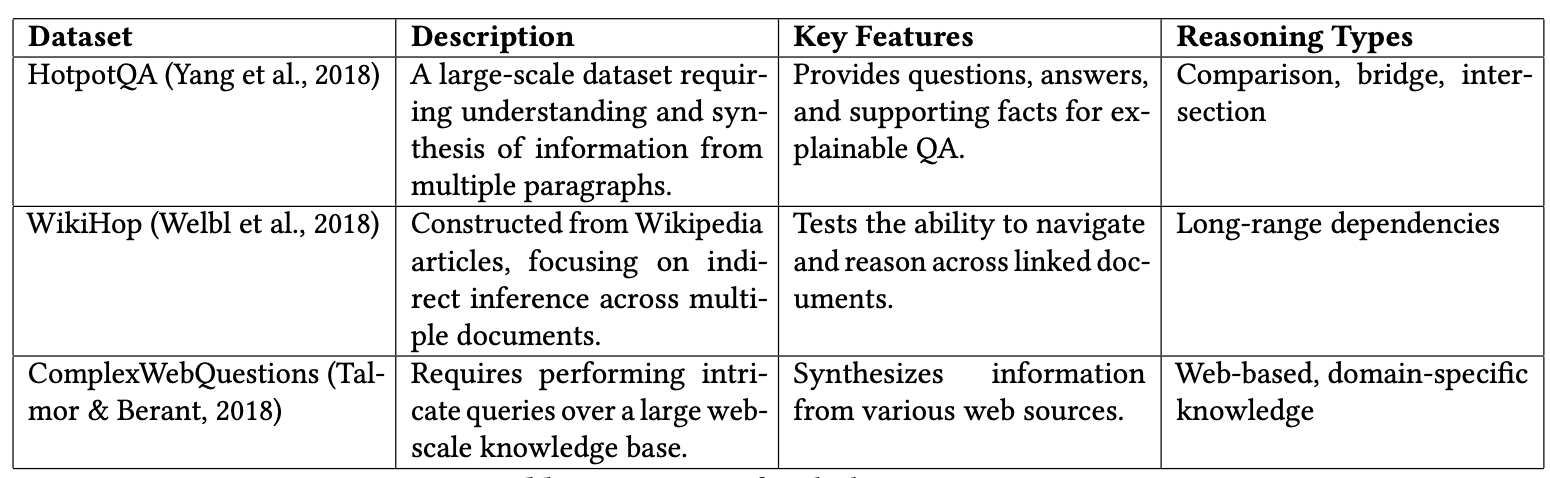
\includegraphics[width=\linewidth]{fig/ext_fig/sample_datasets.png} % Adjust 'width' as needed
    \caption{Sample datasets}
    \label{fig:sample_datasets} % For referencing the figure in the text
  \end{figure}

\end{frame}


\section{Taxonomy}

\begin{frame}[fragile]{Graph Representation}
  \begin{itemize}
    \item Li et al. (2021) \cite{RN131} introduced an Asynchronous Multi-grained Graph Network (AMGN) that represents entities and sentences as nodes, using an asynchronous update mechanism to mimic human multi-hop reading logic.
    \item Tu et al. (2019) \cite{RN124} proposed a Heterogeneous Document-Entity (HDE) graph, where entities are represented as nodes and relationships as edges, and used GNNs for reasoning over this graph.
    \item Zhang et al. (2020) \cite{RN170} presented a context based Entity Graph Convolutional Network (CEG) that also represents entities as nodes, using various granularity levels of encodings and surrounding context 
to enrich entity encoding.
    \item Gao et al. (2023) \cite{RN136} introduced ClueReader, a heterogeneous graph attention network that represents entities as nodes and relationships as edges, and uses an attention mechanism to assemble semantic features in multi-angle representations.
  \end{itemize}
\end{frame}

\begin{frame}[fragile]{Graph Construction}
  \begin{itemize}
    \item Graph neural networks can be considered either static or dynamic.
    \item Discussions in the field of GNNs primarily involve dynamic GNNs.
    \item One approach called Keywords-aware Dynamic Graph Neural Network (KA-DGN) suggested by Jia et al. (2022) \cite{RN171b} emphasizes salient information in the text, extracting keywords from the question and context to improve MHRC performance.
    \item The dynamic structure, in this case, allows for more adaptive and responsive handling of complex questions and multiple paragraphs.
  \end{itemize}
\end{frame}

\begin{frame}[fragile]{Message Passing}
  \begin{itemize}
    \item Graph Message passing enables the integration and reasoning of information scattered across multiple documents.
    \item Aggregation techniques focus on nodes gathering information from adjacent nodes.
    \item Combination practices involve nodes updating their states by combining their own features with the aggregated information.
  \end{itemize}
\end{frame}

\begin{frame}[fragile]{GNN Architectures}
  \begin{itemize}
    \item ConvGNNs utilize a convolutional process on graphs where the focus is on aggregating information from a node's immediate neighbors.
    \item Graph processing can also be done in a recurrent manner, allowing for the capture of information from wider graph neighborhoods over iterations, as displayed by the Recurrent Graph Neural Networks (RGNNs) architecture.
    \item Attention-based Graph Neural Networks are a popular architecture concept for selective focus on important nodes and edges in order to emphasize key information.
    \item Recent advancements include hybrid models that combine different GNN architectures or integrate GNNs with other neural network types for enhanced performance.
  \end{itemize}
\end{frame}

\begin{frame}[fragile]{Dataset and Task Type}
  \begin{itemize}
    \item The ability of GNNs to handle different types of questions and datasets makes them particularly versatile for MHRC tasks.
    \item Specifically for factoid question answering, GNNs are used to connect disparate pieces of information from various texts to answer these questions \cite{RN116}.
    \item Complex reasoning tasks require synthesizing information from various sources to answer questions that involve inference, deduction, or contradiction.
  \end{itemize}
\end{frame}

\begin{frame}[fragile]{Evaluation and Performance Metrics}
  \begin{itemize}
    \item Evaluation of models on the HotpotQA dataset demonstrate accuracy metrics such as F1 score and Exact Match \cite{RN116}.
    \item Interpretability metrics assess how well the model's decision-making process can be understood which is crucial for reliability reasons.
  \end{itemize}
\end{frame}

\begin{frame}[fragile]{Application Domains}
  \begin{itemize}
    \item The flexibility of GNNs in handling different types of data makes them suitable for both domain-specific and general-purpose MHRC.
    \item An example for domain-specific application includes the use of GNNs in biomedical literature for MHRC tasks \cite{RN129}.
    \item A study on the use of GNNs in the HotpotQA dataset, a general-purpose MHRC benchmark, illustrates their effectiveness also in broader applications \cite{RN116}.
  \end{itemize}
\end{frame}

\section{Core Concepts}

\subsection{Graph based approach: HGN}

\begin{frame}
  \frametitle{Hierarchical Graph Network}
  \begin{itemize}
    % \pause
    \item A hierarchical graph network with nodes for different granularity levels, like questions, paragraphs, sentences, and entities. %\pause
    \item Large-scale pre-trained language models like BERT or RoBERTa are used to encode the input text. %\pause
    \item Encoded representations are then used to construct the hierarchical graph. %\pause
    \item Multi-task prediction module performs multiple roles like paragraph selection, supporting fact selection, entity prediction and answer span extraction.
  \end{itemize}

\end{frame}

\begin{frame}
  \frametitle{Hierarchical Graph Network}

  \begin{figure}[t] % 'h' for "here", can be replaced with other placement specifiers
    \centering
    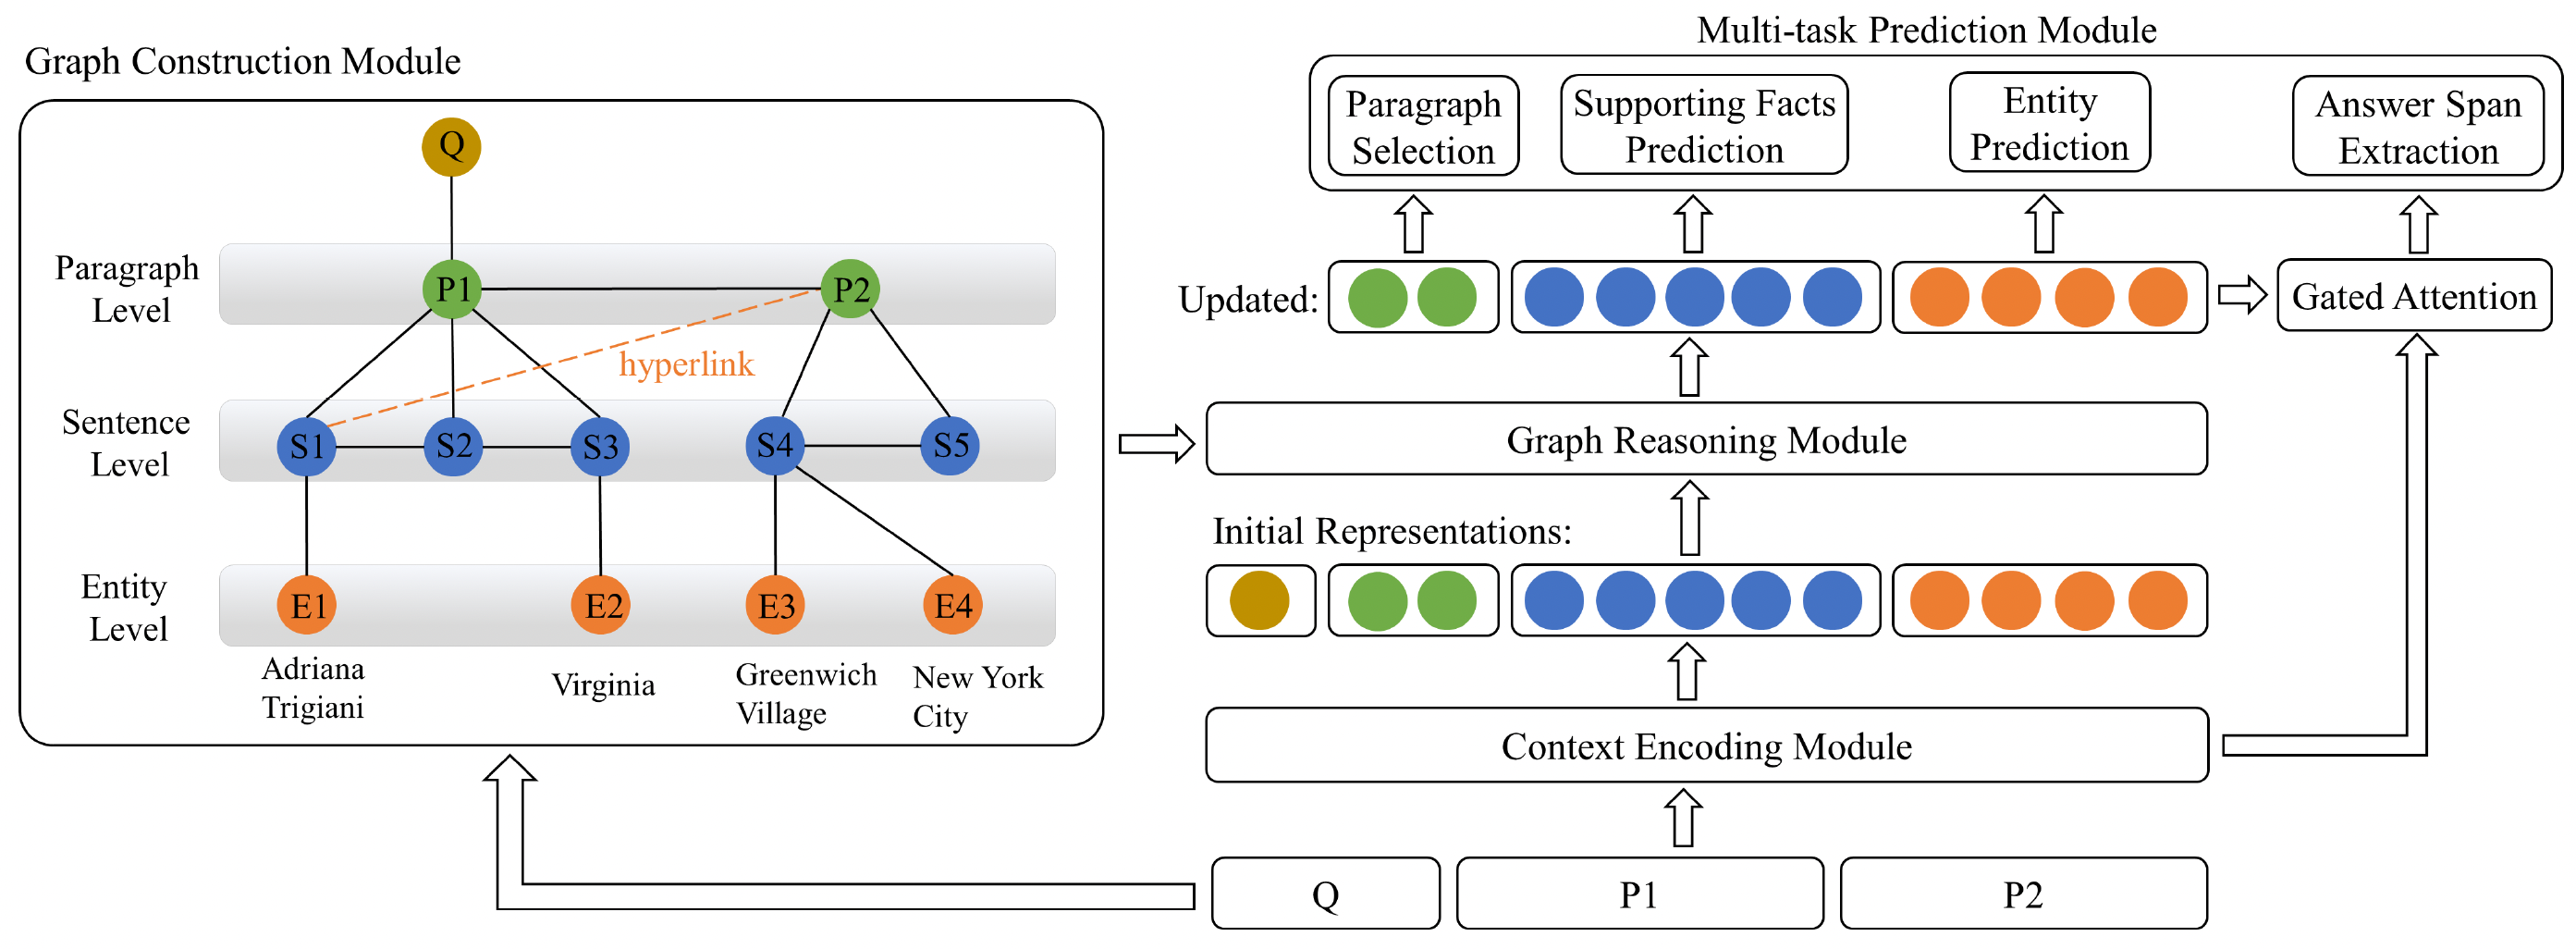
\includegraphics[width=\linewidth]{fig/ext_fig/hgn_diagram.png} % Adjust 'width' as needed
    \caption{Model architecture for HGN, figure taken from \cite{RN119}}
    \label{fig:sample_hotpotqa} % For referencing the figure in the text
  \end{figure}

\end{frame}

\subsection{Non-Graph based approach: S2G}

\begin{frame}
  \frametitle{Select-to-Guide Strategy}

  \begin{columns}
    \begin{column}{0.5\textwidth}  
      \begin{figure}
      \begin{center}
       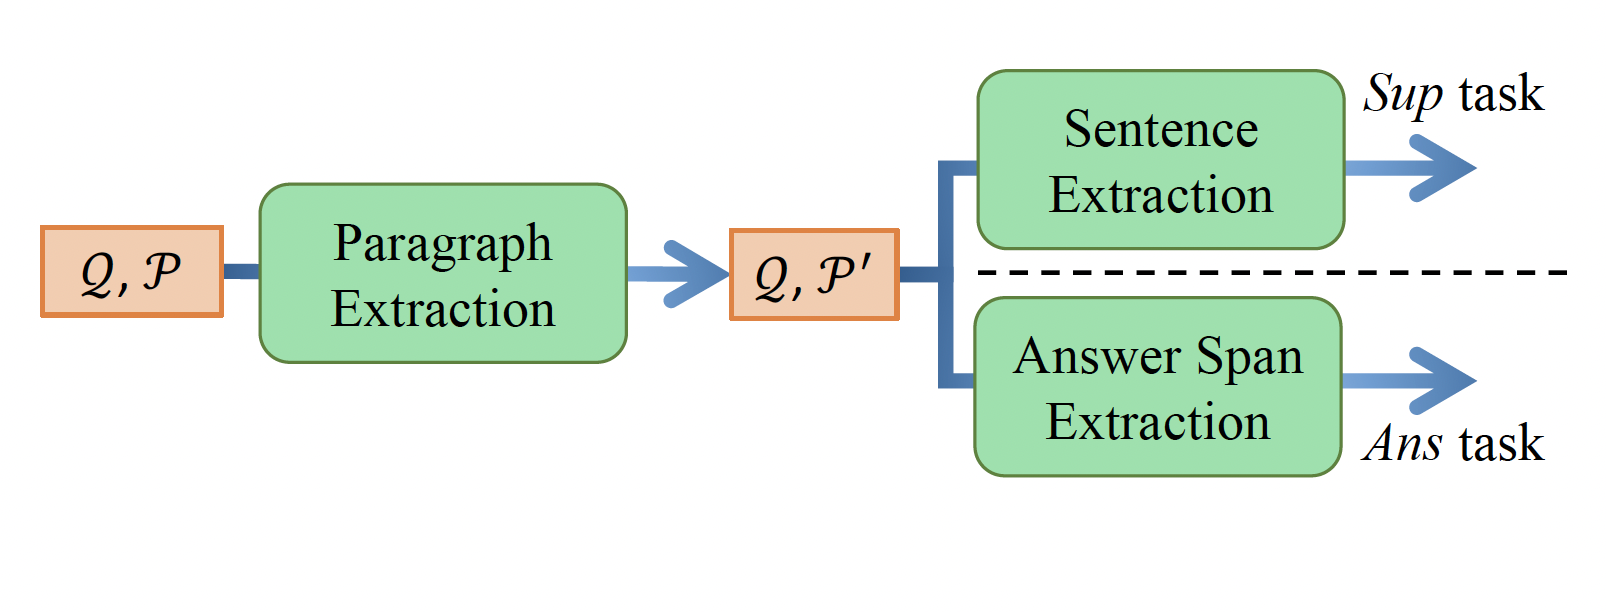
\includegraphics[width=\textwidth]{fig/ext_fig/s2g_pipeline.png}
       \caption{S2G Pipeline, figure taken from \cite{RN106}}
       \end{center}
      \end{figure}
  \end{column}
    \begin{column}{0.5\textwidth}
      \begin{itemize}
        % \pause
        \item Coarse-to-fine, step-wise method for evidence paragraph retrieval. %\pause
        \item Incorporates two novel attention mechanisms for sentence extraction and answer span extraction.
      \end{itemize}
    \end{column}
  \end{columns}

\end{frame}

\begin{frame}
  \frametitle{Select-to-Guide Strategy}

  \begin{figure}[t] % 'h' for "here", can be replaced with other placement specifiers
    \centering
    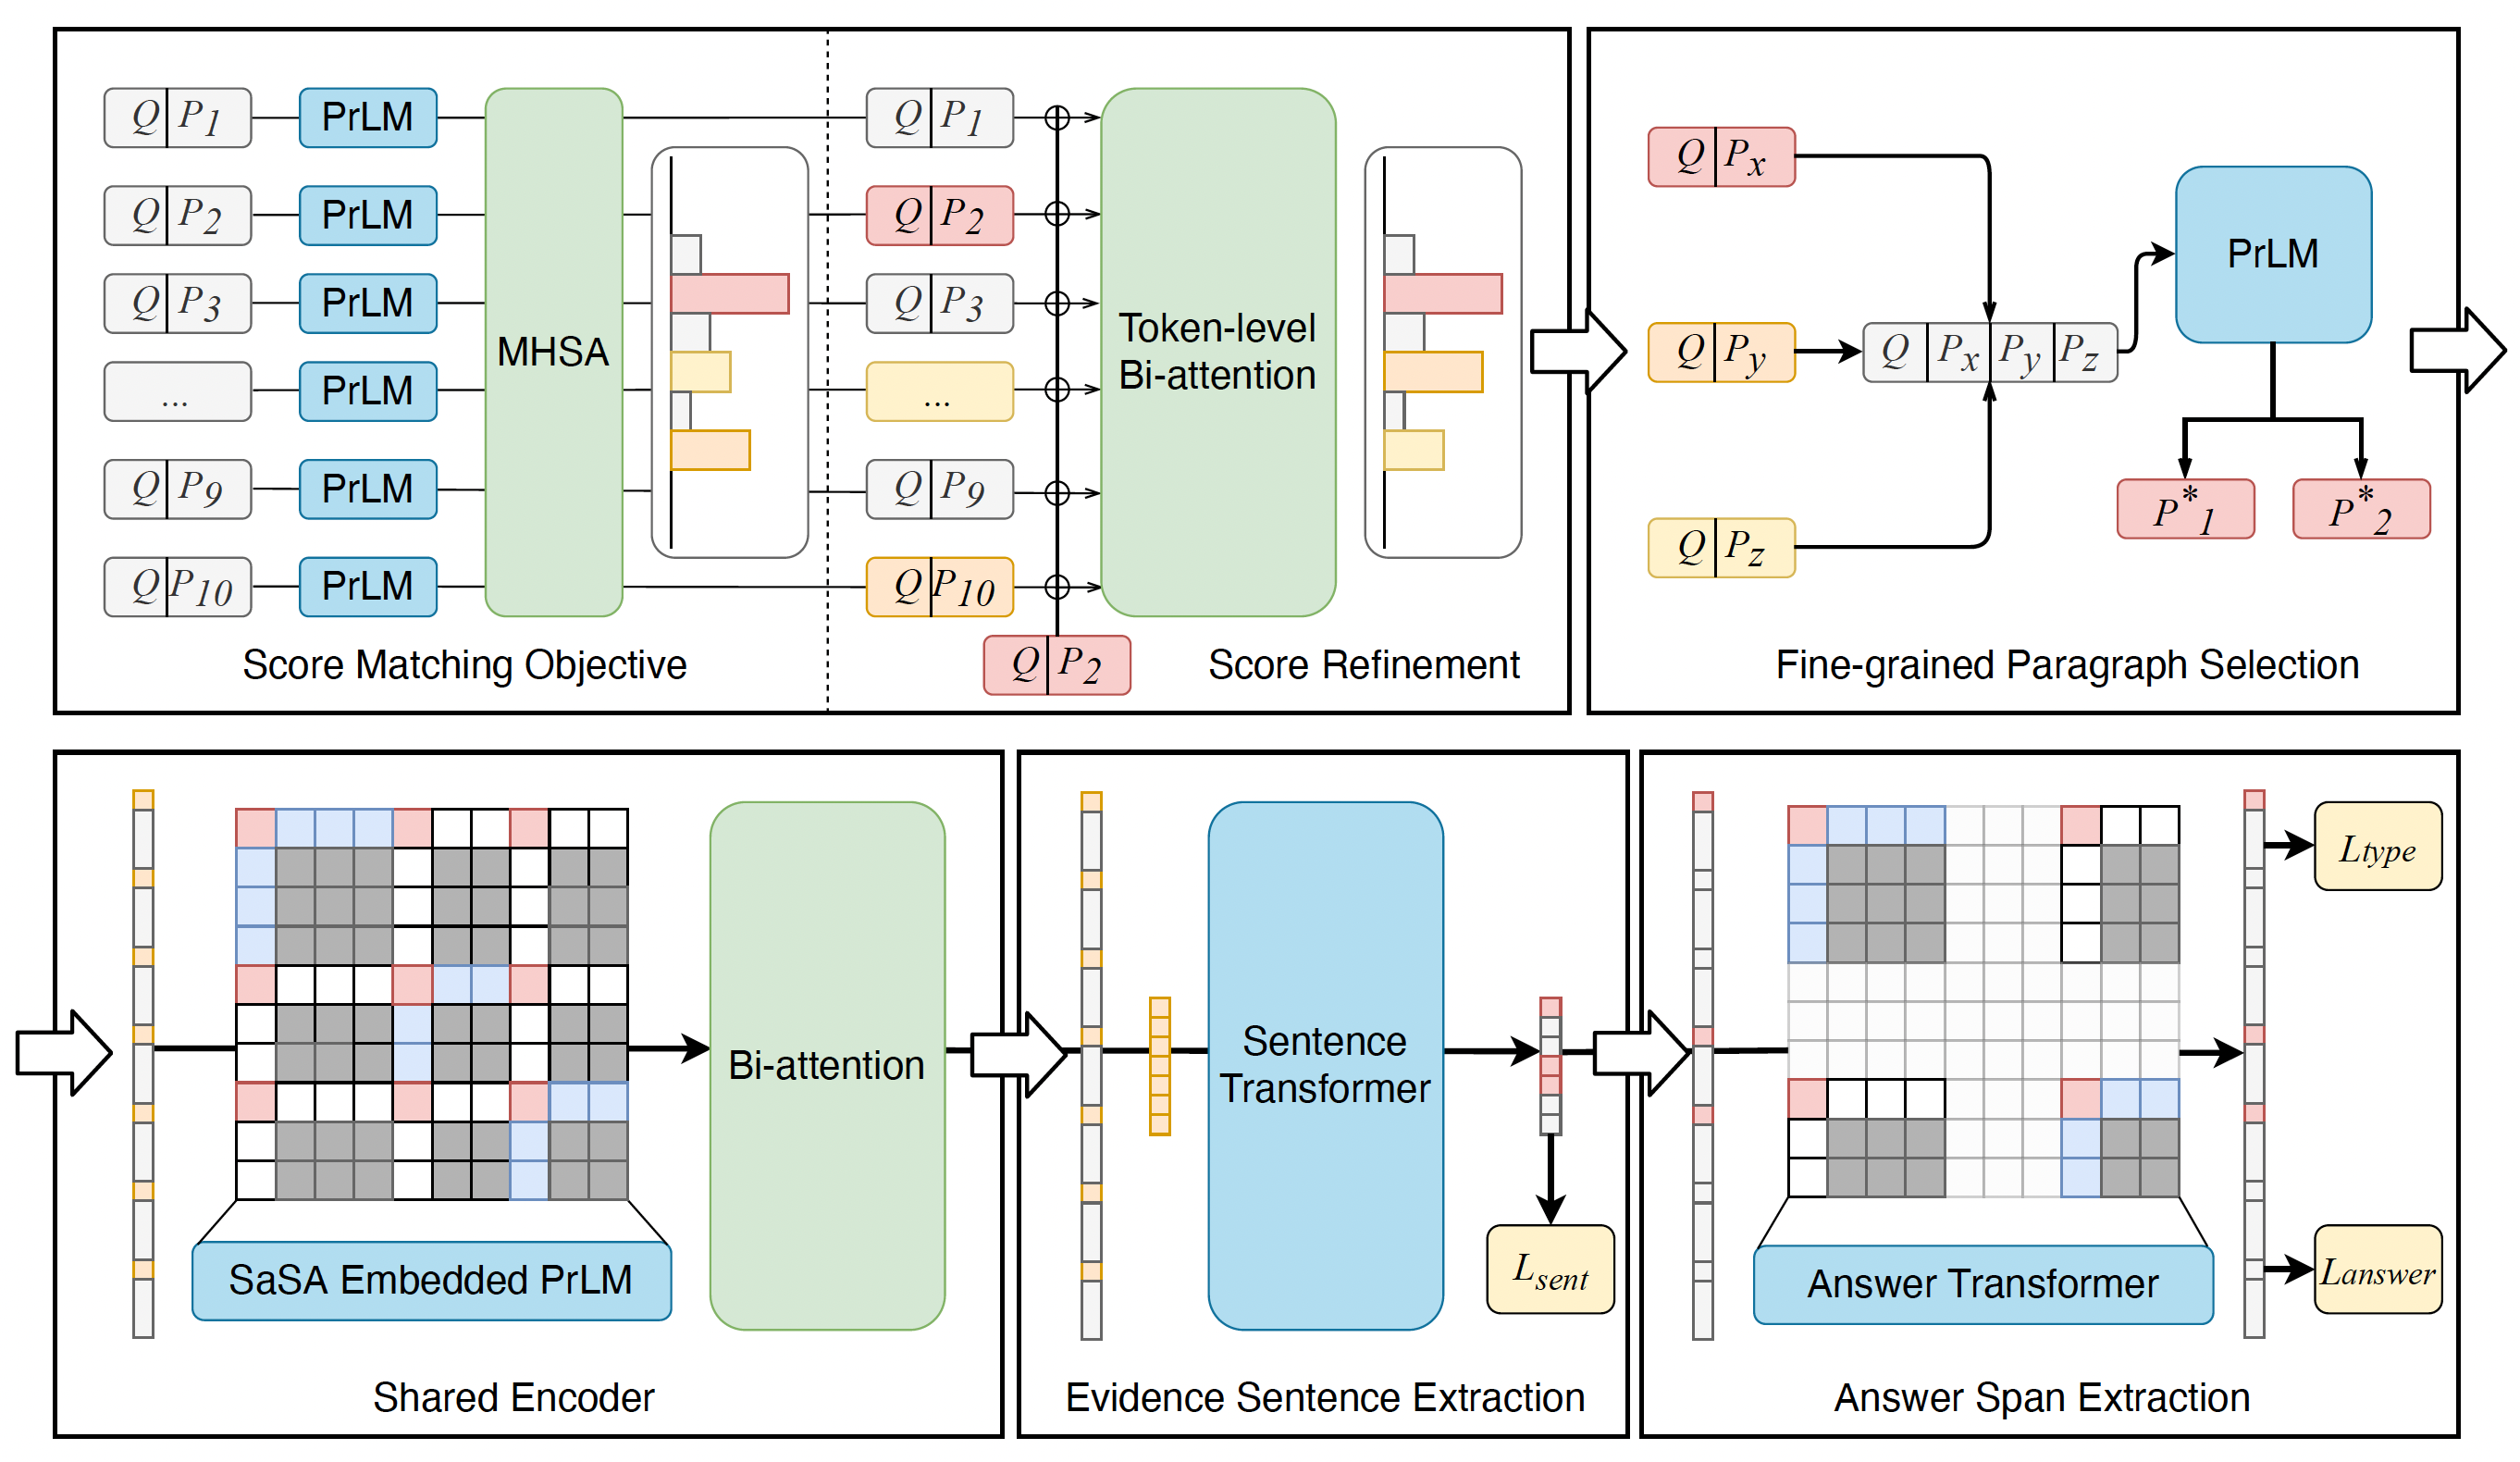
\includegraphics[width=\linewidth]{fig/ext_fig/s2g_diagram.png} % Adjust 'width' as needed
    \caption{Model architecture for S2G, figure taken from \cite{RN106}}
    \label{fig:sample_hotpotqa} % For referencing the figure in the text
  \end{figure}

\end{frame}

\subsection{Arguments against Graph-based approaches}

\begin{frame}
  \frametitle{Arguments against Graph-based approaches}
  \begin{itemize}
    \item \textbf{Shao et al. (2020)} \cite{RN127} argue that with the proper use of pre-trained models, graph structure may not be necessary. %\pause
    \item They also point out that adjacency matrix and graph structure can be regarded as task-related prior knowledge. %\pause
    \item \textbf{Groeneveld et al. (2020)} \cite{RN126} showed that a simple BERT based model can outperform a Graph-based model on the HotpotQA dataset.
  \end{itemize}

\end{frame}

\begin{frame}
  \frametitle{Arguments against Graph-based approaches}
  \begin{itemize}
    \item \textbf{Wu et al. (2021)} \cite{RN106} highlights limitations of graph modeling for MHRC, which requires NER and also rigid rule-based graph construction. %\pause
    \item They also point out that the retrieval stage might be more important than the reasoning stage.
  \end{itemize}

\end{frame}

\subsection{Dataset Limitations}

\begin{frame}
  \frametitle{Dataset Limitations}
  \begin{itemize}
    \item \textbf{Min et al. (2019)} \cite{RN150} argue that constructing large multihop datasets is difficult, and that the current datasets like HotpotQA can be solved with single-hop approaches. %\pause
    \item They noted that humans could solve over 80\% of HotpotQA questions with one gold paragraph withheld.% \pause
    \item \textbf{Groenveld et al. (2020)} \cite{RN126} indicate that HotpotQA might not be suitable to demonstrate the value of more complex retrieval techniques, and that supporting sentence identification in HotpotQA might not be a multi-hop problem at all.% \pause
    \item Several studies \cite{RN154} \cite{RN176} \cite{RN150} \cite{RN175} indicate that many questions in HotpotQA can be answered using heuristics, 
    as they have biases and reasoning shortcuts \cite{RN177}.
  \end{itemize}
  
\end{frame}

% \begin{frame}[fragile]{Typography}
%       \begin{verbatim}The theme provides sensible defaults to
% \emph{emphasize} text, \alert{accent} parts
% or show \textbf{bold} results.\end{verbatim}

%   \begin{center}becomes\end{center}

%   The theme provides sensible defaults to \emph{emphasize} text,
%   \alert{accent} parts or show \textbf{bold} results.
% \end{frame}

% \begin{frame}{Font feature test}
%   \begin{itemize}
%     \item Regular
%     \item \textit{Italic}
%     \item \textsc{SmallCaps}
%     \item \textbf{Bold}
%     \item \textbf{\textit{Bold Italic}}
%     \item \textbf{\textsc{Bold SmallCaps}}
%     \item \texttt{Monospace}
%     \item \texttt{\textit{Monospace Italic}}
%     \item \texttt{\textbf{Monospace Bold}}
%     \item \texttt{\textbf{\textit{Monospace Bold Italic}}}
%   \end{itemize}
% \end{frame}

% \begin{frame}{Lists}
%   \begin{columns}[T,onlytextwidth]
%     \column{0.33\textwidth}
%       Items
%       \begin{itemize}
%         \item Milk \item Eggs \item Potatos
%       \end{itemize}

%     \column{0.33\textwidth}
%       Enumerations
%       \begin{enumerate}
%         \item First, \item Second and \item Last.
%       \end{enumerate}

%     \column{0.33\textwidth}
%       Descriptions
%       \begin{description}
%         \item[PowerPoint] Meeh. \item[Beamer] Yeeeha.
%       \end{description}
%   \end{columns}
% \end{frame}
% \begin{frame}{Animation}
%   \begin{itemize}[<+- | alert@+>]
%     \item \alert<4>{This is\only<4>{ really} important}
%     \item Now this
%     \item And now this
%   \end{itemize}
% \end{frame}
% \begin{frame}{Figures}
%   \begin{figure}
%     \newcounter{density}
%     \setcounter{density}{20}
%     \begin{tikzpicture}
%       \def\couleur{alerted text.fg}
%       \path[coordinate] (0,0)  coordinate(A)
%                   ++( 90:5cm) coordinate(B)
%                   ++(0:5cm) coordinate(C)
%                   ++(-90:5cm) coordinate(D);
%       \draw[fill=\couleur!\thedensity] (A) -- (B) -- (C) --(D) -- cycle;
%       \foreach \x in {1,...,40}{%
%           \pgfmathsetcounter{density}{\thedensity+20}
%           \setcounter{density}{\thedensity}
%           \path[coordinate] coordinate(X) at (A){};
%           \path[coordinate] (A) -- (B) coordinate[pos=.10](A)
%                               -- (C) coordinate[pos=.10](B)
%                               -- (D) coordinate[pos=.10](C)
%                               -- (X) coordinate[pos=.10](D);
%           \draw[fill=\couleur!\thedensity] (A)--(B)--(C)-- (D) -- cycle;
%       }
%     \end{tikzpicture}
%     \caption{Rotated square from
%     \href{http://www.texample.net/tikz/examples/rotated-polygons/}{texample.net}.}
%   \end{figure}
% \end{frame}
% \begin{frame}{Tables}
%   \begin{table}
%     \caption{Largest cities in the world (source: Wikipedia)}
%     \begin{tabular}{lr}
%       \toprule
%       City & Population\\
%       \midrule
%       Mexico City & 20,116,842\\
%       Shanghai & 19,210,000\\
%       Peking & 15,796,450\\
%       Istanbul & 14,160,467\\
%       \bottomrule
%     \end{tabular}
%   \end{table}
% \end{frame}
% \begin{frame}{Blocks}
%   Three different block environments are pre-defined and may be styled with an
%   optional background color.

%   \begin{columns}[T,onlytextwidth]
%     \column{0.5\textwidth}
%       \begin{block}{Default}
%         Block content.
%       \end{block}

%       \begin{alertblock}{Alert}
%         Block content.
%       \end{alertblock}

%       \begin{exampleblock}{Example}
%         Block content.
%       \end{exampleblock}

%     \column{0.5\textwidth}

%       \metroset{block=fill}

%       \begin{block}{Default}
%         Block content.
%       \end{block}

%       \begin{alertblock}{Alert}
%         Block content.
%       \end{alertblock}

%       \begin{exampleblock}{Example}
%         Block content.
%       \end{exampleblock}

%   \end{columns}
% \end{frame}
% \begin{frame}{Math}
%   \begin{equation*}
%     e = \lim_{n\to \infty} \left(1 + \frac{1}{n}\right)^n
%   \end{equation*}
% \end{frame}
% \begin{frame}{Line plots}
%   \begin{figure}
%     \begin{tikzpicture}
%       \begin{axis}[
%         mlineplot,
%         width=0.9\textwidth,
%         height=6cm,
%       ]

%         \addplot {sin(deg(x))};
%         \addplot+[samples=100] {sin(deg(2*x))};

%       \end{axis}
%     \end{tikzpicture}
%   \end{figure}
% \end{frame}
% \begin{frame}{Bar charts}
%   \begin{figure}
%     \begin{tikzpicture}
%       \begin{axis}[
%         mbarplot,
%         xlabel={Foo},
%         ylabel={Bar},
%         width=0.9\textwidth,
%         height=6cm,
%       ]

%       \addplot plot coordinates {(1, 20) (2, 25) (3, 22.4) (4, 12.4)};
%       \addplot plot coordinates {(1, 18) (2, 24) (3, 23.5) (4, 13.2)};
%       \addplot plot coordinates {(1, 10) (2, 19) (3, 25) (4, 15.2)};

%       \legend{lorem, ipsum, dolor}

%       \end{axis}
%     \end{tikzpicture}
%   \end{figure}
% \end{frame}
% \begin{frame}{Quotes}
%   \begin{quote}
%     Veni, Vidi, Vici
%   \end{quote}
% \end{frame}

% {%
% \setbeamertemplate{frame footer}{My custom footer}
% \begin{frame}[fragile]{Frame footer}
%     \themename defines a custom beamer template to add a text to the footer. It can be set via
%     \begin{verbatim}\setbeamertemplate{frame footer}{My custom footer}\end{verbatim}
% \end{frame}
% }

% \begin{frame}{References}
%   Some references to showcase [allowframebreaks] \cite{RN2}
% \end{frame}

\section{Future Directions and Conclusion}

\begin{frame}{Future Research Directions}
  \begin{itemize}
    \item \textbf{Dataset Development:}
      \begin{itemize}
        \item Future datasets should mirror real-world complexity.
        \item Focus on diversity in scenarios, question types, and complexity.
      \end{itemize}
    \item \textbf{Model Efficiency and Generalization:}
      \begin{itemize}
        \item Address computational resource requirements of GNNs.
        \item Promote cross-domain generalization and adaptability.
        \item Explore Hybrid Models combining various GNN architectures.
      \end{itemize}
    \item \textbf{Ethical and Explainable AI:}
      \begin{itemize}
        \item Emphasize transparent decision-making processes.
        \item Focus on making MHRC models more interpretable.
      \end{itemize}
  \end{itemize}
\end{frame}

\begin{frame}{Conclusion}
  \begin{itemize}
    \item GNNs have significantly advanced MHRC by modeling complex textual relationships.
    \item Challenges remain in dataset quality, model scalability, and explainability.
    \item Future research should focus on creating diverse datasets, enhancing model efficiency, and ensuring ethical AI practices.
    \item The synergy between cognitive science and GNNs could pave the way for more intuitive and effective MHRC models.
  \end{itemize}
\end{frame}




% \begin{frame}{Summary}

%   Get the source of this theme and the demo presentation from

%   \begin{center}\url{github.com/matze/mtheme}\end{center}

%   The theme \emph{itself} is licensed under a
%   \href{http://creativecommons.org/licenses/by-sa/4.0/}{Creative Commons
%   Attribution-ShareAlike 4.0 International License}.

%   \begin{center}\ccbysa\end{center}

% \end{frame}

{\setbeamercolor{palette primary}{fg=black, bg=yellow}
\begin{frame}[standout]
  Questions?
\end{frame}
}

\appendix

% \begin{frame}[fragile]{Backup slides}
%   Sometimes, it is useful to add slides at the end of your presentation to
%   refer to during audience questions.

%   The best way to do this is to include the \verb|appendixnumberbeamer|
%   package in your preamble and call \verb|\appendix| before your backup slides.

%   \themename will automatically turn off slide numbering and progress bars for
%   slides in the appendix.
% \end{frame}

\begin{frame}[allowframebreaks]{References}

  \bibliography{bib.bib}
  \bibliographystyle{abbrv}

\end{frame}

\end{document}
